% homework/q1sci/q1sci.tex
% Year 7 - Quarter 1 Review Packet: Science Units 1 and 2, all of it.
%
% Goes out before the Science Quarter 1 Assessment (50 marks, 60 minutes,
% Units 1 and 2 mixed). The assessment lives OUTSIDE this repo, in
% OneDrive\Desktop\Y7Tests\Science\Q1-Assessment, because this repo is public.
% At the teacher's request this packet shares a LITTLE with it: some question
% types, never the same item. Which ones is recorded with the assessment, not
% here. If you edit either, check the packet has not become its answer sheet.
%
% It also borrows, on purpose, from the Cambridge Stage 7 END-OF-YEAR paper:
% the questions on it that Units 1 and 2 can answer, rewritten with new items
% so the class meets the format before June without meeting the paper. A1
% (cell part to job), C3 (a list of symbols and formulae), C5(b) (word to
% statement), C6 (acid or alkali?) and C7 (the particle equation, and the
% two-bottle neutralisation investigation, with the products left out -- not
% taught until Stage 8).
%
% Nothing untaught is asked (see the assessment's header for the list): pH is
% 1 to 14, only litmus colours are words, only a magnet and evaporating
% separate a mixture, no sublimation, only the first 20 elements.
%
% THE LEVELS, as in q1rev: Focus (the basics), Practice (what most of the
% assessment looks like), Challenge (its hardest questions, and harder).
%
% Contexts already used in HW 1-8 are avoided (the syringes, the sponge, the
% puddle, iron and sulfur, the eight pH liquids, Co and CO ...). 2.3 and 2.4
% had no homework before this packet, so B4 and B5 are written at length.
%
% PAGE BREAKS. The first draft was 13 pages; README.md lists what came out.
% Several blocks are minipages on purpose (A2's diagram, A3's list and table,
% each B4 part, C1's box and table, C4(b), C7's word help with question 1, all
% of D1): each was once split across a page. The order inside Sections A and B
% was chosen so the big blocks pack -- a reorder moves every break after it.
%
% House style is shared: see homework/hw-style.tex. Headings are the green of
% the Extra packets (EX 3-8), at the teacher's request. Method: the
% new-homework skill. Source is pure ASCII on purpose.
%
% Build:  pwsh .claude/skills/new-homework/scripts/build-hw.ps1 q1sci

\documentclass[12pt,a4paper]{article}

% -- Answer key switch -------------------------------------------------------
\newif\ifkey
\ifdefined\TEACHER\keytrue\else
  \keyfalse        % \keyfalse = student copy   |   \keytrue = teacher copy
\fi

% -- House style -------------------------------------------------------------
% homework/hw-style.tex
% Shared house style for every Year 7 homework packet. \input this from the
% packet file, right after \documentclass and the answer-key switch.
%
% Do not fork this file per packet. If a packet needs a different look, the
% question is whether every packet should have it.
%
% The choices here are deliberate and were arrived at by printing and looking:
%   * No solid dark banners. Every header is a light tint with a coloured spine
%     on the left, so colour reads clearly without flooding a school printer.
%   * No marks and no mark totals. These are practice, not exam papers.
%   * Lato at 12pt with open leading, plus mathastext so inline maths is Lato
%     too. Without mathastext every "-6 + 4" is Computer Modern serif and the
%     sheet looks half-typeset.
%   * Writing lines are spaced for Year 7 handwriting, not adult margin notes.
%   * Pages fill. \needspace is redefined below so a heading no longer drags
%     the page break up to itself, and every heading is glued to the box under
%     it. Packets built before 2026-09-30 were laid out under the old rules and
%     will reflow if rebuilt -- re-read every page if you rebuild one.
%
% Provides: \wlines \blank \tickbox \sep \qmk-free marks (none) \hwsection
% \qhead \expr, the workspace box, and the remember / wordhelp / activity /
% yourturn coloured boxes. Palette matches the lesson decks exactly.

% -- Packages ----------------------------------------------------------------
\usepackage[T1]{fontenc}
\usepackage[utf8]{inputenc}
\usepackage[default]{lato}
\usepackage[a4paper,top=1.7cm,bottom=1.7cm,left=2.0cm,right=2.0cm,headheight=15pt]{geometry}
\usepackage{amsmath,amssymb}
\usepackage{xcolor}
\usepackage[most]{tcolorbox}
\usepackage{enumitem}
\usepackage{tikz}
\usetikzlibrary{arrows.meta}
\usepackage{array}
\usepackage{tabularx}
\usepackage{fancyhdr}
\usepackage{multicol}
\usepackage{needspace}
\usepackage{graphicx}

% Make maths use Lato too. Without this, every "-6 + 4" on the page is set in
% Computer Modern serif and the sheet looks half-typeset. Must come last.
\usepackage[italic]{mathastext}

% -- \needspace, without the hole it used to leave ----------------------------
% needspace.sty writes "\vskip 0pt plus X \penalty-100" in front of every
% heading. A page that ends anywhere else is underfull with no stretch, so TeX
% scores it b=10000; a page that ends AT a heading gets that X of stretch and a
% finite badness, and wins. So any heading in roughly the bottom half of a page
% claimed the break, and the question under it moved over whole, leaving a hole
% the size of the question. \tracingpages showed it exactly (b=4531 at the
% heading, b=10000 at every later break) while building homework/q1rev, and it
% is where the half-empty pages in HW 1-8 came from.
% This keeps only the \penalty9999, which still refuses to put a heading in the
% last X of a page. Keeping a heading WITH the box under it is \nobreak's job
% now -- see \hwsection and \qhead below.
\makeatletter
\renewcommand{\needspace}[1]{\begingroup\setlength{\dimen@}{#1}%
  \vskip\dimen@\penalty9999\vskip-\dimen@\endgroup}
\makeatother

\linespread{1.06}\selectfont

% -- The Learner's Book palette (same hex values as the lesson decks) ---------
\definecolor{cbteal}{HTML}{0087A8}
\definecolor{cbpurple}{HTML}{5C2483}
\definecolor{cborange}{HTML}{C25E12}
\definecolor{cbgreen}{HTML}{4A8B23}
\definecolor{cbred}{HTML}{C8102E}
\definecolor{cbblue}{HTML}{1A5FA8}
\definecolor{rulegray}{HTML}{9AA5AD}

% -- Answer lines and blanks -------------------------------------------------
% \wlines{n} draws n ruled writing lines, spaced wide enough for Year 7
% handwriting rather than for an adult with a fine pen.
\makeatletter
\newcommand{\wlines}[1]{%
  \par\vspace{0.75em}%
  \@tempcnta=0\relax
  \@whilenum\@tempcnta<#1\do{%
    \hbox to \linewidth{\color{rulegray}\leaders\hrule height 0.5pt\hfill}%
    \vspace{1.5em}%
    \advance\@tempcnta by 1\relax}%
  \par\vspace{-0.8em}%
}
\makeatother

% \blank[width] is an inline gap to write a short answer in.
\newcommand{\blank}[1][2.6cm]{\underline{\hspace{#1}}}

% A boxed space for showing working.
\newtcolorbox{workspace}[1][3.4cm]{%
  colback=white, colframe=rulegray, boxrule=0.5pt, arc=5pt,
  height=#1, left=6pt, right=6pt, top=4pt, bottom=4pt,
  before skip=9pt, after skip=11pt}

% An empty tick box.
\newcommand{\tickbox}{\fbox{\rule{0pt}{1.15em}\rule{1.15em}{0pt}}}

% A middot separator.
\newcommand{\sep}{\,\textperiodcentered\,}

% -- Section and question headings -------------------------------------------
% Light tint plus a fat coloured spine on the left. No solid dark banner: the
% colour reads clearly but barely costs the printer anything.
% needspace keeps a heading out of the last few lines of a page. The \nobreak
% after it keeps it with whatever comes next: a remember or word-help box that
% does not fit takes its heading over with it, instead of leaving the heading
% alone at the foot of the page. (The old needspace did that by accident, and
% left a hole every time; see above.)
\newcommand{\hwsection}[2][cbteal]{%
  \needspace{8\baselineskip}%
  \par\vspace{13pt}%
  \noindent
  \begin{tcolorbox}[enhanced, nobeforeafter, width=\textwidth,
      colback=#1!7, colframe=#1!7, arc=5pt,
      borderline west={5pt}{0pt}{#1},
      left=14pt, right=10pt, top=7pt, bottom=7pt]
    {\large\bfseries\color{#1}#2}
  \end{tcolorbox}%
  \par\nobreak\vspace{9pt}}

% \qhead[colour]{A2}{Moving along the line} -- a question heading.
\newcommand{\qhead}[3][cbteal]{%
  \needspace{6\baselineskip}%
  \par\vspace{11pt}%
  \noindent{\large\bfseries\color{#1}#2}\quad{\large\bfseries #3}\par\nobreak\vspace{4pt}}

% -- Coloured boxes ----------------------------------------------------------
% Shared look: rounded, light fill, coloured rule, coloured title text on a
% pale title strip rather than a dark one.
% NOT breakable. A breakable box that cannot fit its first lines forces its own
% page break, and \nobreak cannot stop a forced break -- so the heading above
% it was left alone at the foot of the page (tested: it happens with \nobreak
% in place). Unbreakable, the page builder moves heading and box together.
% These boxes are a few lines each; none needs to split.
\tcbset{hwbox/.style={
  enhanced, arc=6pt, boxrule=1pt,
  left=11pt, right=11pt, top=8pt, bottom=8pt,
  fonttitle=\bfseries, attach boxed title to top left={xshift=12pt, yshift=-8pt},
  boxed title style={arc=4pt, boxrule=1pt, left=7pt, right=7pt, top=2pt, bottom=2pt},
  top=13pt}}

% Orange: things to remember. Matches the deck's "Write This Down".
\newtcolorbox{remember}[1][Remember from the lesson]{hwbox,
  colback=cborange!6, colframe=cborange, coltitle=cborange,
  colbacktitle=white, title={#1}}

% Blue: English help. The barrier in this class is the wording, not the maths.
\newtcolorbox{wordhelp}[1][Word help]{hwbox,
  colback=cbblue!6, colframe=cbblue, coltitle=cbblue,
  colbacktitle=white, title={#1}}

% Purple: an activity or instruction.
\newtcolorbox{activity}[1][How to do this homework]{hwbox,
  colback=cbpurple!6, colframe=cbpurple, coltitle=cbpurple,
  colbacktitle=white, title={#1}}

% Green: your turn / a friendly nudge.
\newtcolorbox{yourturn}[1][Your turn]{hwbox,
  colback=cbgreen!7, colframe=cbgreen, coltitle=cbgreen!75!black,
  colbacktitle=white, title={#1}}

% -- Shorthands --------------------------------------------------------------
\newcommand{\dC}{\,^{\circ}\mathrm{C}}          % use inside maths: $-8\dC$
\newcommand{\key}[1]{{\color{cborange}\textbf{#1}}}
\newcommand{\eng}[1]{{\color{cbblue}\textbf{#1}}}

\setlist[enumerate]{itemsep=8pt, topsep=5pt, leftmargin=*}
\setlist[itemize]{itemsep=4pt, topsep=4pt, leftmargin=*}
\renewcommand{\arraystretch}{1.45}

% -- An expression the student is asked to work from -------------------------
\newcommand{\expr}[1]{%
  \tcbox[on line, colback=cbgreen!10, colframe=cbgreen!55, boxrule=1pt, arc=4pt,
         left=9pt, right=9pt, top=4pt, bottom=4pt]{\large\bfseries $#1$}}

% -- Running head and foot ---------------------------------------------------
% The packet overrides \fancyhead[L] with its own title.
\pagestyle{fancy}
\fancyhf{}
\fancyhead[L]{\small\color{black!55}Year 7\sep Homework}
\fancyhead[R]{\small\color{black!55}Name: \blank[3.4cm]}
\fancyfoot[C]{\small\color{black!55}Page \thepage}
\renewcommand{\headrulewidth}{0pt}
\renewcommand{\headrule}{\vspace{2pt}\hbox to\headwidth{\color{cbteal!45}\leaders\hrule height 1.2pt\hfill}}


\usetikzlibrary{calc,decorations.pathmorphing}
\usepackage{colortbl}   % \cellcolor, for the metals in C2

% -- Per-packet running head -------------------------------------------------
% No name line on every page: the name goes once, on the cover. The rule under
% the head is green to match the headings.
\fancyhead[L]{\small\color{black!55}Year 7\sep Science Q1 Review}
\fancyhead[R]{}
\renewcommand{\headrule}{\vspace{2pt}\hbox to\headwidth{\color{cbgreen!45}\leaders\hrule height 1.2pt\hfill}}

% -- Writing lines that will not be split -------------------------------------
\newcommand{\qlines}[1]{\par\needspace{\numexpr#1+1\relax\baselineskip}\wlines{#1}}

% -- A ragged-right X column --------------------------------------------------
\newcolumntype{L}{>{\raggedright\arraybackslash}X}
\newcolumntype{C}[1]{>{\centering\arraybackslash}p{#1}}

% -- The three levels (as q1rev) ----------------------------------------------
\newcommand{\levtag}[2]{%
  \tcbox[on line, colback=white, colframe=#1, boxrule=0.9pt, arc=3pt,
         left=5pt, right=5pt, top=1.5pt, bottom=1.5pt]%
        {\footnotesize\bfseries\color{#1}#2}}
\newcommand{\focus}{\levtag{cbgreen}{FOCUS}}
\newcommand{\practice}{\levtag{cbteal}{PRACTICE}}
\newcommand{\challenge}{\levtag{cbred}{CHALLENGE}}
% \evq{A1}{Title}{\focus} -- a green question heading carrying its level.
\newcommand{\evq}[3]{\qhead[cbgreen]{#1}{#2\hfill#3}}

% -- Chemistry ----------------------------------------------------------------
\newcommand{\ch}[1]{\ensuremath{\mathrm{#1}}}
\newcommand{\ccm}{\ensuremath{\mathrm{cm^3}}}

% A sentence starter: grey, so it reads as given, not as the answer.
\newcommand{\starter}[1]{{\color{black!60}#1}}

% An answer blank on a line of its own, right-aligned (see hw08.tex).
\newcommand{\ansline}[1][4.4cm]{\par\vspace{2pt}\hspace*{\fill}\blank[#1]\par}

% A box to write one number in.
\newcommand{\nbox}{\ \fbox{\rule{0pt}{1.05em}\rule{1.0em}{0pt}}\ }

% A table row tall enough to write in.
\newcommand{\tall}{\rule[-0.75em]{0pt}{2.2em}}

% Atom colours are the 2.6 deck's: O red, S yellow, and a plain grey/white
% pair where the element does not matter.
\tikzset{
  atomD/.style={circle, draw=black!75, fill=black!55, line width=0.6pt,
                minimum size=#1, inner sep=0pt},
  atomD/.default=0.34cm,
  atomL/.style={circle, draw=black!75, fill=white, line width=0.6pt,
                minimum size=#1, inner sep=0pt},
  atomL/.default=0.34cm}

\begin{document}

% ===========================================================================
% COVER BLOCK
% ===========================================================================
\thispagestyle{fancy}

\begin{tcolorbox}[enhanced, colback=cbgreen!8, colframe=cbgreen!8, arc=7pt,
                  borderline west={6pt}{0pt}{cbgreen},
                  left=18pt, right=14pt, top=11pt, bottom=11pt]
  {\color{cbgreen!75!black}\bfseries YEAR 7\sep SCIENCE}\\[5pt]
  {\color{cbgreen!70!black}\Huge\bfseries Q1 Review: Science Units 1 and 2}\\[9pt]
  {\color{black!70}Science 1.1--1.4 --- cells, specialised cells, tissues and organs}\\
  {\color{black!70}Science 2.1--2.4 --- particles, changes of state, the water cycle}\\
  {\color{black!70}Science 2.5--2.8 --- atoms, compounds, mixtures, acids and bases}
\end{tcolorbox}

\vspace{4pt}
\noindent
\begin{tabularx}{\textwidth}{@{}X X@{}}
  \textbf{Name:} \blank[5.6cm] & \textbf{Date given:} \blank[4.6cm] \\
\end{tabularx}

\vspace{2pt}
\begin{activity}[How to use this packet]
  {\color{cbgreen}\bfseries Focus} the basics \sep
  {\color{cbteal}\bfseries Practice} like the assessment \sep
  {\color{cbred}\bfseries Challenge} the hardest --- do not skip \\
  \key{Answer in full sentences.} ``Nucleus'' is not a sentence.
\end{activity}

% ===========================================================================
% SECTION A -- UNIT 1
% ===========================================================================
\hwsection[cbgreen]{Section A \textperiodcentered\ Unit 1 --- Cells, Tissues and Organs}

% -- A1 ---------------------------------------------------------------------
% After end-of-year Q2 (four parts to four jobs); here all seven, and two of the
% jobs both start with "controls" -- the English trap.
\evq{A1}{Every part has a job}{\focus}

\begin{wordhelp}[Word help --- two parts both ``control'' something]
  \eng{controls} --- is in charge of. \quad \eng{releases} --- lets out. \quad
  Read the words \textbf{after} ``controls'': \emph{what goes in and out} is one
  part; \emph{everything the cell does} is another.
\end{wordhelp}

\noindent\textbf{(a)} Draw \textbf{one} line from each part of a cell to its job.

\vspace{6pt}
\begin{center}
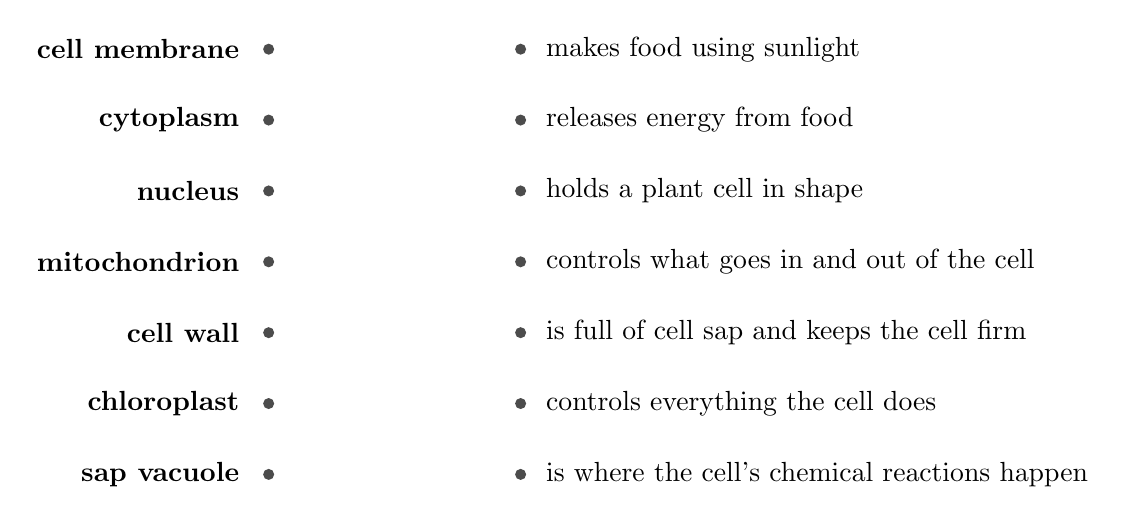
\begin{tikzpicture}[x=1cm, y=1cm,
    pl/.style={anchor=east, font=\normalsize},
    jb/.style={anchor=west, font=\normalsize}]
  \foreach \t [count=\i] in {cell membrane, cytoplasm, nucleus, mitochondrion,
                             cell wall, chloroplast, sap vacuole}{
    \node[pl] at (3.9,-0.9*\i) {\textbf{\t}};
    \fill[black!70] (4.15,-0.9*\i) circle (0.07);}
  \foreach \t [count=\i] in {makes food using sunlight,
                             releases energy from food,
                             holds a plant cell in shape,
                             controls what goes in and out of the cell,
                             is full of cell sap and keeps the cell firm,
                             controls everything the cell does,
                             is where the cell's chemical reactions happen}{
    \fill[black!70] (7.35,-0.9*\i) circle (0.07);
    \node[jb] at (7.55,-0.9*\i) {\t};}
\end{tikzpicture}
\end{center}

\noindent\textbf{(b)} Draw a ring around the \textbf{three} parts in (a) that an
\textbf{animal} cell does \textbf{not} have.

% -- A2 ---------------------------------------------------------------------
% The root hair cell has never been labelled on a packet (HW 1 did a plant
% cell, HW 5 an animal cell). The wall band is 0.35 thick so the wall (1) and
% the membrane (2) are clearly two lines, as HW 1 insists.
\evq{A2}{The root hair cell}{\practice}

% The instruction and the diagram are one block: apart, the heading and the
% instruction were left at the foot of page 1.
\noindent
\begin{minipage}{\textwidth}
\noindent\textbf{(a)} Write the name of each numbered part.

\vspace{4pt}
\noindent
\begin{minipage}[c]{0.62\textwidth}
\resizebox{\linewidth}{!}{%
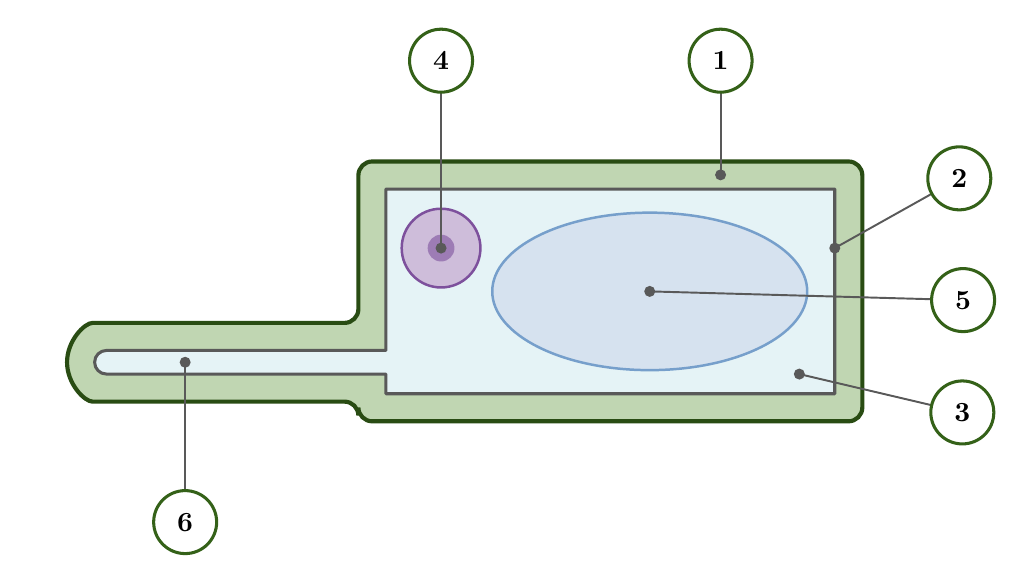
\begin{tikzpicture}[x=1cm, y=1cm,
    lbl/.style={circle, draw=cbgreen!70!black, fill=white, line width=1.1pt,
                inner sep=1.8pt, minimum size=8mm, font=\bfseries}]
  % the wall (outer) and the membrane (inner), body and hair as one outline
  \fill[cbgreen!35, rounded corners=5pt]
    (4,3.3) -- (10.4,3.3) -- (10.4,0) -- (4,0) -- (4,0.25) -- (0.8,0.25)
    arc (270:90:0.5) -- (4,1.25) -- cycle;
  % The inner line has no "rounded corners": on the small arc at the tip of the
  % hair they fought each other and drew a jagged notch.
  \fill[cbteal!10]
    (4.35,2.95) -- (10.05,2.95) -- (10.05,0.35) -- (4.35,0.35) -- (4.35,0.6)
    -- (0.8,0.6) arc (270:90:0.15) -- (4.35,0.9) -- cycle;
  \draw[black!65, line width=1.1pt, line join=round]
    (4.35,2.95) -- (10.05,2.95) -- (10.05,0.35) -- (4.35,0.35) -- (4.35,0.6)
    -- (0.8,0.6) arc (270:90:0.15) -- (4.35,0.9) -- cycle;
  \draw[cbgreen!55!black, line width=1.5pt, rounded corners=5pt]
    (4,3.3) -- (10.4,3.3) -- (10.4,0) -- (4,0) -- (4,0.25) -- (0.8,0.25)
    arc (270:90:0.5) -- (4,1.25) -- cycle;
  % the sap vacuole, and the nucleus near the root hair
  \fill[cbblue!18] (7.7,1.65) ellipse (2.0 and 1.0);
  \draw[cbblue!60, line width=0.9pt] (7.7,1.65) ellipse (2.0 and 1.0);
  \fill[cbpurple!30] (5.05,2.2) circle (0.5);
  \draw[cbpurple!80, line width=0.9pt] (5.05,2.2) circle (0.5);
  \fill[cbpurple!60] (5.05,2.2) circle (0.17);
  % leaders, each ending on a dot
  \foreach \sx/\sy/\ex/\ey/\n in {%
      8.6/3.13/8.6/4.2/1,        % cell wall: the green band
      10.05/2.2/11.3/2.9/2,      % cell membrane: the dark line
      9.6/0.6/11.3/0.2/3,        % cytoplasm: the corner patch
      5.05/2.2/5.05/4.2/4,       % nucleus
      7.7/1.65/11.3/1.55/5,      % sap vacuole
      1.8/0.75/1.8/-0.9/6}{      % root hair
    \draw[line width=0.7pt, black!65] (\sx,\sy) -- (\ex,\ey);
    \fill[black!65] (\sx,\sy) circle (0.07);
    \node[lbl] at ($(\ex,\ey)!-0.38cm!(\sx,\sy)$) {\n};}
  \path (-0.2,-1.6) rectangle (12.0,4.9);
\end{tikzpicture}}
\end{minipage}\hfill
\begin{minipage}[c]{0.35\textwidth}
  \renewcommand{\arraystretch}{2.0}%
  \begin{tabular}{@{}l@{\ }l@{}}
    1 & \blank[4.4cm] \\
    2 & \blank[4.4cm] \\
    3 & \blank[4.4cm] \\
    4 & \blank[4.4cm] \\
    5 & \blank[4.4cm] \\
    6 & \blank[4.4cm] \\
  \end{tabular}
\end{minipage}
\end{minipage}

\vspace{8pt}
\noindent\textbf{(b)} Water from the soil goes into the cell. Number these
\textbf{1 to 4} in the order the water passes through them.

\vspace{6pt}
\noindent\hspace*{1.2em}\nbox cell membrane \qquad \nbox sap vacuole \qquad
\nbox cell wall \qquad \nbox cytoplasm

\vspace{10pt}
\noindent\textbf{(c)} Why does this cell have a long, thin root hair? \\
\starter{The long root hair gives the cell \ldots}
\qlines{2}

% -- A3 ---------------------------------------------------------------------
\evq{A3}{Which level is it?}{\focus}

\begin{remember}[Each level is built out of the one before it]
  \key{cell} $\rightarrow$ \key{tissue} (similar cells, one job) $\rightarrow$
  \key{organ} (several tissues) $\rightarrow$ \key{organ system} (organs, one shared
  job) $\rightarrow$ \key{organism}
\end{remember}

\noindent
\begin{minipage}{\textwidth}
Write each one in the correct column.

\vspace{4pt}
\begin{center}
  a neurone \sep the brain \sep ciliated epithelium \sep a mango tree \sep the
  digestive system \\[2pt]
  a root \sep the palisade layer \sep a red blood cell \sep the breathing system \sep a cat
\end{center}

\vspace{2pt}
\noindent
\begin{tabularx}{\textwidth}{|X|X|X|X|X|}
  \hline
  \textbf{Cell} & \textbf{Tissue} & \textbf{Organ} & \textbf{Organ system} &
  \textbf{Organism} \\ \hline
  \rule{0pt}{4.4em} & & & & \\ \hline
\end{tabularx}
\end{minipage}

% -- A4 ---------------------------------------------------------------------
\evq{A4}{Mr Bowen's table has four mistakes}{\practice}

\noindent There is \textbf{one} mistake in each row. Cross it out and write the correct
words next to it.

\vspace{6pt}
\noindent
{\renewcommand{\arraystretch}{1.3}%
\begin{tabularx}{\textwidth}{|p{2.6cm}|L|L|}
  \hline
  \textbf{Cell} & \textbf{Function} & \textbf{Special structure} \\ \hline
  red blood cell & carries oxygen & has a very long axon \rule[-1.6em]{0pt}{3.2em} \\ \hline
  neurone & carries electrical signals & has a large sap vacuole \rule[-1.6em]{0pt}{3.2em} \\ \hline
  ciliated cell & absorbs water from the soil & has cilia (tiny hairs) \rule[-1.6em]{0pt}{3.2em} \\ \hline
  palisade cell & makes food by photosynthesis & has no nucleus \rule[-1.6em]{0pt}{3.2em} \\ \hline
\end{tabularx}}

% -- A5 ---------------------------------------------------------------------
% Three of the 1.1-1.3 ideas no packet has asked: how small a cell is (Unit 3
% maths, dividing by 0.02), what a model gets wrong, and the white blood cell
% exit question.
\evq{A5}{Unit 1 puzzles}{\challenge}

\begin{wordhelp}[Word help]
  \eng{side by side} --- in a line, touching. \quad
  \eng{squeezes} --- pushes through a small space.
\end{wordhelp}

\noindent
\begin{minipage}{\textwidth}
  \textbf{1.} A typical human cell is $0.02$ mm across.
  \par\vspace{3pt}
  (a) How many cells, side by side, make a line 1 mm long? \hfill \blank[2.4cm] \\[5pt]
  (b) How many make a line 1 cm long? \hfill \blank[2.4cm] \\[5pt]
  (c) A hair is $0.07$ mm thick. About how many cells wide is it? \hfill \blank[2.4cm]
\end{minipage}

\vspace{12pt}
\noindent
\begin{minipage}{\textwidth}
  \textbf{2.} A white blood cell chases germs, squeezes between other cells and
  swallows the germs. Why would a cell wall be \textbf{no good} to it?
  \wlines{2}
\end{minipage}

% ===========================================================================
% SECTION B -- UNIT 2: PARTICLES AND CHANGES OF STATE
% ===========================================================================
\hwsection[cbgreen]{Section B \textperiodcentered\ Unit 2 --- Particles, Changes of State, the Water Cycle}


% -- B1 ---------------------------------------------------------------------
\evq{B1}{Draw the particles}{\focus}

\noindent Draw about 12 particles in each box. Use circles of the same size.

\vspace{6pt}
\begin{center}
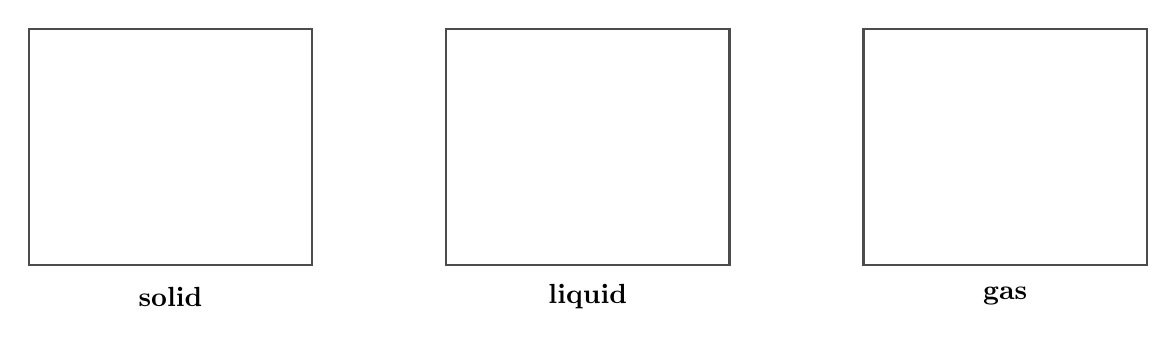
\begin{tikzpicture}
  \foreach \x/\t in {0/solid, 5.3/liquid, 10.6/gas}{
    \draw[thick, black!70] (\x,0) rectangle (\x+3.6,3.0);
    \node[font=\bfseries] at (\x+1.8,-0.4) {\t};}
\end{tikzpicture}
\end{center}

% -- B2 ---------------------------------------------------------------------
\evq{B2}{Solid, liquid or gas?}{\focus}

% The instruction is the table's own header row (as q1rev A5 and B1), so it
% cannot be left at the foot of a page while the table goes over.
\noindent
\begin{tabularx}{\textwidth}{|L|C{1.7cm}|C{1.7cm}|C{1.7cm}|}
  \hline
  \textbf{Tick every state it is true for. Some rows need two ticks.} &
  \textbf{Solid} & \textbf{Liquid} & \textbf{Gas} \\ \hline
  It keeps its own shape. \tall & & & \\ \hline
  It fills any closed container. \tall & & & \\ \hline
  It takes the shape of its container, but keeps the same volume. \tall & & & \\ \hline
  It can be poured. \tall & & & \\ \hline
  It cannot be compressed. \tall & & & \\ \hline
  The particles vibrate, but stay in the same place. \tall & & & \\ \hline
  The particles touch, but can move past one another. \tall & & & \\ \hline
\end{tabularx}

% -- B3 ---------------------------------------------------------------------
\evq{B3}{Name the change}{\practice}

\begin{remember}[Five changes of state]
  \key{melting} solid $\rightarrow$ liquid \sep \key{freezing} liquid $\rightarrow$ solid
  \sep \key{evaporating} and \key{boiling} liquid $\rightarrow$ gas \sep
  \key{condensing} gas $\rightarrow$ liquid
\end{remember}

\noindent
\begin{tabularx}{\textwidth}{|L|p{3.6cm}|C{2.6cm}|}
  \hline
  \textbf{What happens} & \textbf{Change of state} & \textbf{Heating or cooling?} \\ \hline
  A bar of chocolate goes soft in a hot car. \tall & & \\ \hline
  Mr Bowen breathes on a cold window. Drops of water appear. \tall & & \\ \hline
  Melted butter goes hard in the fridge. \tall & & \\ \hline
  A wet floor dries in the afternoon. \tall & & \\ \hline
  Water in a kettle bubbles at $100\dC$. \tall & & \\ \hline
\end{tabularx}

% -- B4 ---------------------------------------------------------------------
% 2.3 had no homework before this packet. Boiling, condensing and expanding
% were taught from the front with no copy-down, so this is the first time the
% class writes them.
\evq{B4}{Explain it with particles}{\practice}

% No remember box here: the sentence starters carry the same ideas, and the box
% alone was left at the foot of page 4 with both parts on page 5.
% Each part is a minipage, so a question and its starter cannot sit at the foot
% of one page with their lines on the next.
\noindent
\begin{minipage}{\textwidth}
\textbf{(a)} What happens to the particles when water boils? \\
\starter{Heat energy is transferred to \ldots\ The particles move \ldots\ Some of them
escape \ldots}
\wlines{3}
\end{minipage}

\vspace{8pt}
\noindent
\begin{minipage}{\textwidth}
\textbf{(b)} Drops of water form on the outside of a cold can of drink. Where do
they come from? \\
\starter{There is water vapour in \ldots\ When it touches the cold can, the particles
\ldots}
\wlines{3}
\end{minipage}

% -- B5 ---------------------------------------------------------------------
% 2.4 had no homework before this packet: all six arrows the class drew.
\evq{B5}{The water cycle}{\practice}

\noindent\textbf{(a)} Write the name of each numbered arrow. Use the words in the box.

\vspace{4pt}
\begin{center}
  \fbox{\parbox{0.92\linewidth}{\centering\vspace{2pt}
    condensation \qquad evaporation \qquad groundwater \\[3pt]
    precipitation \qquad surface run-off \qquad transpiration\vspace{2pt}}}
\end{center}

\vspace{2pt}
\begin{center}
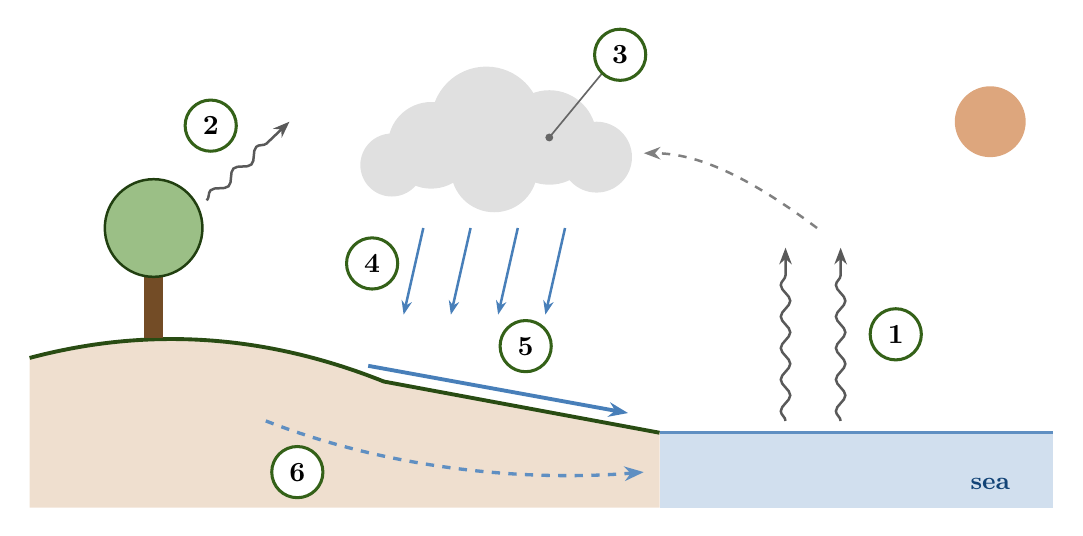
\begin{tikzpicture}[x=1cm, y=1cm, line width=0.9pt,
    lab/.style={circle, draw=cbgreen!70!black, fill=white, line width=1.1pt,
                inner sep=1.5pt, minimum size=6.5mm, font=\bfseries}]
  % the ground: soil, a slope down to the sea
  \fill[brown!25] (0,0) -- (0,1.9) .. controls (1.5,2.3) and (3.0,2.2)
    .. (4.5,1.6) -- (8.0,0.95) -- (8.0,0) -- cycle;
  \draw[cbgreen!55!black, line width=1.4pt] (0,1.9) .. controls (1.5,2.3) and
    (3.0,2.2) .. (4.5,1.6) -- (8.0,0.95);
  \fill[cbblue!20] (8.0,0) rectangle (13,0.95);
  \draw[cbblue!70] (8.0,0.95) -- (13,0.95);
  \node[font=\small\bfseries, text=cbblue!70!black] at (12.2,0.3) {sea};
  % a tree
  \fill[brown!60!black] (1.45,2.15) rectangle (1.7,3.1);
  \fill[cbgreen!55] (1.575,3.55) circle (0.62);
  \draw[cbgreen!45!black] (1.575,3.55) circle (0.62);
  % the sun
  \fill[cborange!55] (12.2,4.9) circle (0.45);
  % the cloud
  \foreach \x/\y/\r in {5.1/4.6/0.55, 5.8/4.9/0.7, 6.6/4.7/0.6, 7.2/4.45/0.45,
                        4.6/4.35/0.4, 5.9/4.3/0.55}{
    \fill[black!12] (\x,\y) circle (\r);}
  % 1 evaporation: from the sea
  \foreach \x in {9.6,10.3}{
    \draw[black!65, -{Stealth[length=6pt]}, decorate,
      decoration={snake, amplitude=0.6mm, segment length=4mm, post length=2mm}]
      (\x,1.1) -- (\x,3.3);}
  \node[lab] at (11.0,2.2) {1};
  % 2 transpiration: from the leaves
  \draw[black!65, -{Stealth[length=6pt]}, decorate,
    decoration={snake, amplitude=0.6mm, segment length=4mm, post length=2mm}]
    (2.25,3.9) -- (3.3,4.9);
  \node[lab] at (2.3,4.85) {2};
  % 3 condensation: at the cloud
  \draw[black!50, dashed, -{Stealth[length=6pt]}] (10.0,3.55) .. controls (9.0,4.3)
    and (8.4,4.5) .. (7.8,4.5);
  \draw[black!60, line width=0.6pt] (6.6,4.7) -- (7.3,5.55);
  \fill[black!60] (6.6,4.7) circle (0.05);
  \node[lab] at (7.5,5.75) {3};
  % 4 precipitation: rain
  \foreach \x in {5.0,5.6,6.2,6.8}{
    \draw[cbblue!80, -{Stealth[length=5pt]}] (\x,3.55) -- (\x-0.25,2.45);}
  \node[lab] at (4.35,3.1) {4};
  % 5 surface run-off: over the ground, down the slope
  \draw[cbblue!80, line width=1.4pt, -{Stealth[length=7pt]}] (4.3,1.8) -- (7.6,1.2);
  \node[lab] at (6.3,2.05) {5};
  % 6 groundwater: through the soil, underneath
  \draw[cbblue!70, line width=1.2pt, dashed, -{Stealth[length=7pt]}] (3.0,1.1)
    .. controls (4.8,0.4) and (6.6,0.35) .. (7.8,0.45);
  \node[lab] at (3.4,0.45) {6};
\end{tikzpicture}
\end{center}

\vspace{2pt}
\noindent
\begin{tabular}{@{}l@{\ }l@{\hspace{0.8cm}}l@{\ }l@{\hspace{0.8cm}}l@{\ }l@{}}
  1 & \blank[3.4cm] & 2 & \blank[3.4cm] & 3 & \blank[3.4cm] \\[12pt]
  4 & \blank[3.4cm] & 5 & \blank[3.4cm] & 6 & \blank[3.4cm] \\
\end{tabular}

\vspace{10pt}
\noindent\textbf{(b)} You can never see water vapour. So what is a cloud made of?
\qlines{2}

\noindent\textbf{(c)} Rain is one kind of precipitation. Name \textbf{two} other kinds.
\hfill \blank[2.6cm] \; \blank[2.6cm]

% -- B6 ---------------------------------------------------------------------
\evq{B6}{Particle puzzles}{\challenge}

% The heating curve from the 2.2b practical, read as a graph. (b) is the trap:
% the kettle is still being heated at 10 minutes.
\noindent
\begin{minipage}{\textwidth}
\noindent
\begin{minipage}[c]{0.485\textwidth}
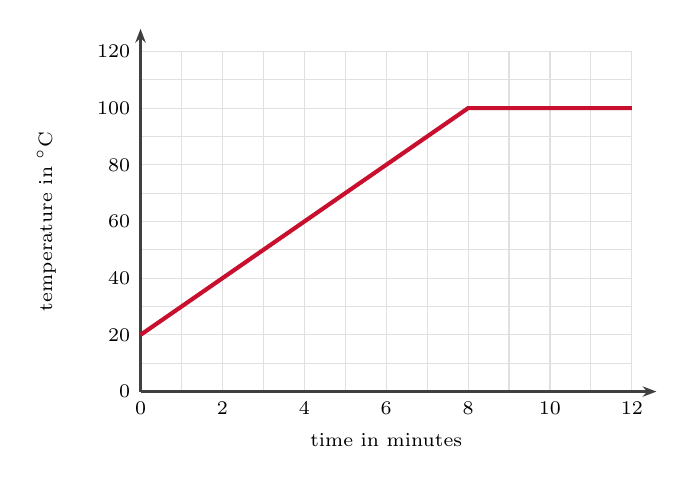
\begin{tikzpicture}[x=0.52cm, y=0.036cm, line width=0.8pt]
  \foreach \t in {0,1,...,12}{\draw[black!12, line width=0.4pt] (\t,0) -- (\t,120);}
  \foreach \T in {0,10,...,120}{\draw[black!12, line width=0.4pt] (0,\T) -- (12,\T);}
  \draw[black!75, -{Stealth[length=5pt]}] (0,0) -- (12.6,0);
  \draw[black!75, -{Stealth[length=5pt]}] (0,0) -- (0,128);
  \foreach \t in {0,2,...,12}{\node[below, font=\scriptsize] at (\t,0) {\t};}
  \foreach \T in {0,20,...,120}{\node[left, font=\scriptsize] at (0,\T) {\T};}
  \node[font=\scriptsize] at (6,-17) {time in minutes};
  \node[font=\scriptsize, rotate=90] at (-2.3,60) {temperature in $^{\circ}$C};
  \draw[cbred, line width=1.5pt] (0,20) -- (8,100) -- (12,100);
\end{tikzpicture}
\end{minipage}\hfill
\begin{minipage}[c]{0.50\textwidth}
  \textbf{1.} Mr Bowen heats a beaker of water for 12 minutes. The graph shows its
  temperature.
  \par\vspace{6pt}
  (a) When does the water start to boil? \\[3pt]
  \hspace*{\fill}\blank[2.8cm]
  \par\vspace{6pt}
  (b) He is still heating it at 10 minutes. What is the temperature? \\[3pt]
  \hspace*{\fill}\blank[2.8cm]
\end{minipage}
\par\vspace{6pt}
\noindent (c) Why does the temperature stop going up, even though he is still heating it?
\wlines{3}
\end{minipage}

\vspace{12pt}
\noindent
\begin{minipage}{\textwidth}
  \textbf{2.} Wet clothes dry faster on a hot, sunny day than on a cold day. Explain
  why, using particles.
  \wlines{3}
\end{minipage}

% ===========================================================================
% SECTION C -- UNIT 2: ATOMS, COMPOUNDS, MIXTURES, ACIDS
% ===========================================================================
\hwsection[cbgreen]{Section C \textperiodcentered\ Unit 2 --- Atoms, Compounds, Mixtures, Acids and Bases}


% -- C1 ---------------------------------------------------------------------
\evq{C1}{Symbols, both ways}{\focus}

% The box and the table are one minipage: apart, the box stayed with the
% heading at the foot of a page and the table went over on its own.
\noindent
\begin{minipage}{\textwidth}
\begin{remember}[The capital-letter rule]
  The first letter is \key{always a capital}. A second letter is \key{always small}:
  Mg, not MG or mg. \; A few come from Latin names: potassium is \key{K}.
\end{remember}

\noindent
\begin{tabularx}{\textwidth}{@{}X X@{}}
  \textbf{(a)} Write the symbol. & \textbf{(b)} Write the name. \\[4pt]
  oxygen \blank[1.6cm] \quad potassium \blank[1.6cm] &
  He \blank[2.4cm] \quad S \blank[2.4cm] \\[10pt]
  magnesium \blank[1.4cm] \quad calcium \blank[1.4cm] &
  Li \blank[2.4cm] \quad Ar \blank[2.4cm] \\[10pt]
  nitrogen \blank[1.6cm] \quad aluminium \blank[1.4cm] &
  F \blank[2.4cm] \quad Si \blank[2.4cm] \\
\end{tabularx}
\end{minipage}

% -- C2 ---------------------------------------------------------------------
% The same 20 elements the class learned, with the metals shaded (the book's
% table colours them yellow). Rows and columns are labelled here, unlike on
% the assessment.
\evq{C2}{Rows and columns}{\practice}

% The word help is the first line of the question column, not a box: a box
% here was left alone at the foot of page 6 with its table on page 7, and
% keeping them together pushed every page after it over.

\noindent
\begin{minipage}[t]{0.53\textwidth}
  \vspace{0pt}
  \renewcommand{\arraystretch}{1.4}%
  \setlength{\tabcolsep}{0pt}%
  \newcommand{\mt}[1]{\cellcolor{cborange!22}#1}%
  \newcommand{\gonem}[1]{\multicolumn{1}{|>{\centering\arraybackslash}p{0.88cm}|}{\cellcolor{cborange!22}#1}}%
  \begin{tabular}{c*{8}{>{\centering\arraybackslash}p{0.88cm}|}}
    \multicolumn{1}{c}{} & \multicolumn{8}{c}{\small\bfseries group} \\
    \multicolumn{1}{c}{} & \multicolumn{1}{c}{\small 1} & \multicolumn{1}{c}{\small 2}
      & \multicolumn{1}{c}{\small 3} & \multicolumn{1}{c}{\small 4}
      & \multicolumn{1}{c}{\small 5} & \multicolumn{1}{c}{\small 6}
      & \multicolumn{1}{c}{\small 7} & \multicolumn{1}{c}{\small 8} \\
    \cline{5-6}\cline{9-9}
    \makebox[1.5cm][r]{\small\bfseries period\ \ 1\ } & \multicolumn{3}{c|}{} &
      \multicolumn{2}{c|}{H} & \multicolumn{2}{c|}{} & He \\ \cline{2-9}
    \makebox[1.5cm][r]{\small 2\ } & \gonem{Li} & \mt{Be} & B & C & N & O & F & Ne \\ \cline{2-9}
    \makebox[1.5cm][r]{\small 3\ } & \gonem{Na} & \mt{Mg} & \mt{Al} & Si & P & S & Cl & Ar \\ \cline{2-9}
    \makebox[1.5cm][r]{\small 4\ } & \gonem{K} & \mt{Ca} & \multicolumn{6}{c}{} \\ \cline{2-3}
  \end{tabular}
  \par\vspace{4pt}
  {\small \colorbox{cborange!22}{\strut\ \ \ } = metal}
\end{minipage}\hfill
\begin{minipage}[t]{0.45\textwidth}
  \vspace{2pt}
  {\small \eng{period} = a \textbf{row} (across), not a lesson \\
          \eng{group} = a \textbf{column} (down), not people}
  \par\vspace{8pt}
  \textbf{(a)} Period 3, group 2: \hfill \blank[1.2cm]
  \par\vspace{10pt}
  \textbf{(b)} Calcium is in period \blank[1.2cm]
  \par\vspace{10pt}
  \textbf{(c)} Two in group 8: \hfill \blank[1.2cm] \ \blank[1.2cm]
  \par\vspace{10pt}
  \textbf{(d)} Li and Na are in the same \hfill \blank[1.8cm]
\end{minipage}

% -- C3 ---------------------------------------------------------------------
% After end-of-year Q9 (Na, O2, Ca, CO2, NaOH, KCl, CaCO3), with a new list.
% (d) is its "contains a metal and carbon" item, which is where -ate lives.
\evq{C3}{Symbols and formulae}{\practice}

\begin{remember}[Reading a formula]
  The small number counts the atom \key{just before it}. No number means \key{one}. \;
  \ch{CO_2} is 1 carbon $+$ 2 oxygen $=$ 3 atoms.
\end{remember}

\begin{center}
  \fbox{\parbox{0.92\linewidth}{\centering\large\vspace{3pt}
    \ch{K} \quad\ \ \ch{Cl_2} \quad\ \ \ch{MgO} \quad\ \ \ch{CH_4} \quad\ \ \ch{Ca}
    \quad\ \ \ch{H_2O} \quad\ \ \ch{NaOH} \quad\ \ \ch{K_2CO_3}\vspace{3pt}}}
\end{center}

\vspace{4pt}
\noindent Choose from the box.
\begin{enumerate}[label=(\alph*), itemsep=9pt]
  \item Write \textbf{two} elements made of single atoms. \hfill \blank[1.4cm] \
        \blank[1.4cm]
  \item Write the element whose particles are \textbf{two atoms} joined together.
        \hfill \blank[1.8cm]
  \item Write the compound that is \textbf{cooking gas}. \hfill \blank[1.8cm]
  \item Write the substance that contains a metal, carbon \textbf{and} oxygen, and
        give its name. \\[3pt]
        \hspace*{\fill}\blank[1.8cm] \quad name: \blank[5.0cm]
  \item How many atoms are in \ch{NaOH}? \blank[1.2cm] \qquad in \ch{K_2CO_3}?
        \blank[1.2cm]
\end{enumerate}

% -- C4 ---------------------------------------------------------------------
\evq{C4}{Naming compounds}{\practice}

\begin{remember}[Two naming rules]
  The \key{metal comes first}, and the non-metal ends in \key{-ide}: sodium $+$
  chlorine $\rightarrow$ sodium chlor\key{ide}. \; Two elements \key{plus oxygen} often
  end in \key{-ate}: calcium carbon\key{ate}.
\end{remember}

\noindent\textbf{(a)} Name the compound made from:

% A table, not multicols: in two columns the fourth item wrapped and its words
% were spread across the line.
\vspace{4pt}
\noindent
\begin{tabular}{@{}l@{\ \ }l@{\hspace{0.6cm}}l@{\ \ }l@{}}
  1. sodium and sulfur & \blank[2.8cm] & 3. lithium and chlorine & \blank[2.8cm] \\[10pt]
  2. oxygen and calcium & \blank[2.8cm] & 4. magnesium, carbon and oxygen &
    \blank[1.9cm] \\
\end{tabular}

% (b) is one block, so its question cannot end a page without its lines.
\vspace{10pt}
\noindent
\begin{minipage}{\textwidth}
\textbf{(b)} Which elements are in each compound?

\vspace{4pt}
\begin{enumerate}[label=\arabic*., itemsep=10pt]
  \item potassium nitrate \hfill \blank[8.4cm]
  \item copper sulfate \hfill \blank[8.4cm]
\end{enumerate}
\end{minipage}

% -- C5 ---------------------------------------------------------------------
% (a) is the Cambridge particle-box format. (b) is end-of-year Q8's
% "one line from each word to a statement", with 2.5-2.7 words.
\evq{C5}{Element, compound or mixture?}{\practice}

\noindent\textbf{(a)} Each circle is an atom. Circles that touch are bonded. Write
\textbf{E} (element), \textbf{C} (compound) or \textbf{M} (mixture) under each box.

\vspace{6pt}
\begin{center}
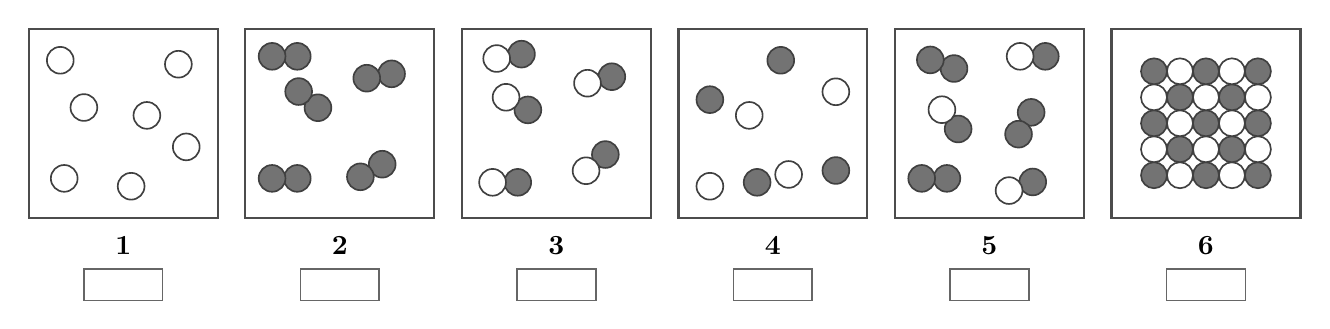
\begin{tikzpicture}[x=1cm, y=1cm]
  \foreach \i in {0,...,5}{
    \draw[thick, black!70] (\i*2.75,0) rectangle (\i*2.75+2.4,2.4);
    \node[font=\bfseries] at (\i*2.75+1.2,-0.35) {\pgfmathparse{int(\i+1)}\pgfmathresult};
    \draw[black!60, line width=0.6pt] (\i*2.75+0.7,-1.05) rectangle (\i*2.75+1.7,-0.65);}
  % 1: single atoms, one kind
  \foreach \x/\y in {0.45/0.5, 1.3/0.4, 2.0/0.9, 0.7/1.4, 1.5/1.3, 0.4/2.0, 1.9/1.95}{
    \node[atomL] at (\x,\y) {};}
  % 2: pairs of the same atom
  \begin{scope}[shift={(2.75,0)}]
    \foreach \x/\y/\a in {0.5/0.5/0, 1.6/0.6/30, 0.8/1.5/-40, 1.7/1.8/10, 0.5/2.05/0}{
      \node[atomD] at ($(\x,\y)+(\a:0.16)$) {};
      \node[atomD] at ($(\x,\y)+(\a+180:0.16)$) {};}
  \end{scope}
  % 3: pairs of two different atoms (all the same compound)
  \begin{scope}[shift={(5.5,0)}]
    \foreach \x/\y/\a in {0.55/0.45/0, 1.7/0.7/40, 0.7/1.45/-30, 1.75/1.75/15, 0.6/2.05/10}{
      \node[atomD] at ($(\x,\y)+(\a:0.16)$) {};
      \node[atomL] at ($(\x,\y)+(\a+180:0.16)$) {};}
  \end{scope}
  % 4: two kinds of single atom, not bonded
  \begin{scope}[shift={(8.25,0)}]
    \foreach \x/\y in {0.4/0.4, 1.4/0.55, 0.9/1.3, 2.0/1.6}{\node[atomL] at (\x,\y) {};}
    \foreach \x/\y in {1.0/0.45, 2.0/0.6, 0.4/1.5, 1.3/2.0}{\node[atomD] at (\x,\y) {};}
  \end{scope}
  % 5: an element (dark pairs) mixed with a compound (dark-light pairs)
  \begin{scope}[shift={(11,0)}]
    \foreach \x/\y/\a in {0.5/0.5/0, 1.65/1.2/60, 0.6/1.95/-20}{
      \node[atomD] at ($(\x,\y)+(\a:0.16)$) {};
      \node[atomD] at ($(\x,\y)+(\a+180:0.16)$) {};}
    \foreach \x/\y/\a in {1.6/0.4/20, 0.7/1.25/-50, 1.75/2.05/0}{
      \node[atomD] at ($(\x,\y)+(\a:0.16)$) {};
      \node[atomL] at ($(\x,\y)+(\a+180:0.16)$) {};}
  \end{scope}
  % 6: a grid of two kinds, alternating, all touching (like salt)
  \begin{scope}[shift={(13.75,0)}]
    \foreach \r in {0,...,4}{\foreach \c in {0,...,4}{
      \pgfmathparse{int(mod(\r+\c,2))}
      \ifnum\pgfmathresult=0 \node[atomD, minimum size=0.33cm] at (0.54+\c*0.33,0.54+\r*0.33) {};
      \else \node[atomL, minimum size=0.33cm] at (0.54+\c*0.33,0.54+\r*0.33) {};\fi}}
  \end{scope}
\end{tikzpicture}
\end{center}

\vspace{6pt}
\noindent\textbf{(b)} Draw \textbf{one} line from each word to what it means.

\vspace{4pt}
\begin{center}
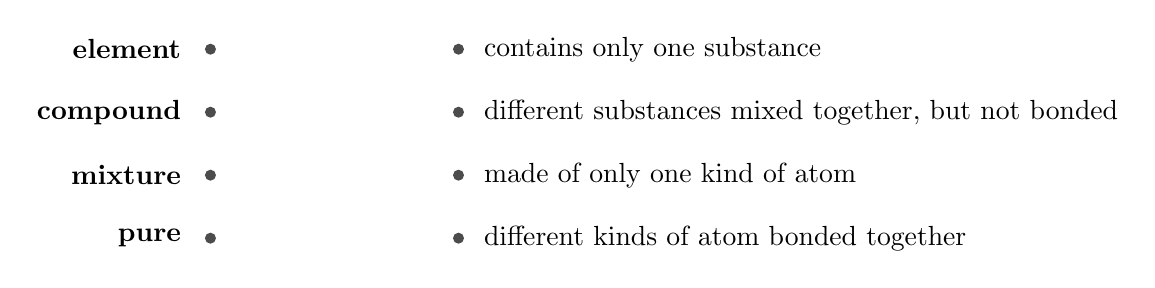
\begin{tikzpicture}[x=1cm, y=1cm]
  \foreach \t [count=\i] in {element, compound, mixture, pure}{
    \node[anchor=east, font=\bfseries] at (2.6,-0.8*\i) {\t};
    \fill[black!70] (2.85,-0.8*\i) circle (0.07);}
  \foreach \t [count=\i] in {contains only one substance,
                             {different substances mixed together, but not bonded},
                             made of only one kind of atom,
                             different kinds of atom bonded together}{
    \fill[black!70] (6.0,-0.8*\i) circle (0.07);
    \node[anchor=west] at (6.2,-0.8*\i) {\t};}
\end{tikzpicture}
\end{center}

\noindent\textbf{(c)} A mixture is easy to separate. How would you get:
\par\vspace{6pt}
\noindent\hspace*{1.2em}the iron filings out of iron filings and sand? \hfill \blank[5.2cm]
\par\vspace{10pt}
\noindent\hspace*{1.2em}the minerals out of mineral water? \hfill \blank[5.2cm]

% -- C6 ---------------------------------------------------------------------
% After end-of-year Q6 (five cards into acid / alkali). Twelve here, all from
% the 2.8 deck's own examples and rules.
\evq{C6}{Acid or alkali?}{\focus}

\begin{remember}[Litmus]
  \key{Blue} litmus turns \key{red} in an acid. \; \key{Red} litmus turns \key{blue}
  in an alkali. \; Below 7 is acid; above 7 is alkali; 7 is neutral.
\end{remember}

\noindent Write each one in the correct column.

\vspace{4pt}
\begin{center}
  tastes sour \sep pH 2 \sep pH 12 \sep turns blue litmus red \sep turns red litmus
  blue \sep tamarind \\[2pt]
  toothpaste \sep stomach acid \sep limewater \sep hydrochloric acid \sep sodium
  hydroxide \sep baking soda
\end{center}

\vspace{2pt}
\noindent
\begin{tabularx}{\textwidth}{|X|X|}
  \hline
  \textbf{Acid} & \textbf{Alkali} \\ \hline
  \rule{0pt}{6.8em} & \\ \hline
\end{tabularx}

% -- C7 ---------------------------------------------------------------------
% Two end-of-year questions. 1 is Q7 (magnesium + oxygen, drawn as particles)
% with sulfur, whose dioxide the 2.6 deck named. 2 is Q10 (two bottles of
% sodium hydroxide) with its products part removed -- salt and water is
% Stage 8 -- and a mean the class can work out without a calculator.
\evq{C7}{Two questions from the end of the year}{\challenge}

% The word help is inside question 1's minipage: outside it, the box stayed
% with the heading at the foot of a page and question 1 went over alone.
\noindent
\begin{minipage}{\textwidth}
  \begin{wordhelp}[Word help]
    \eng{reactants} --- the substances you \textbf{start} with. \quad
    \eng{product} --- the \textbf{new} substance that is made. \\
    \eng{mean} --- add the results, then divide by how many there are.
  \end{wordhelp}
  \textbf{1.} Sulfur burns in oxygen. The picture shows the particles.
  \par\vspace{6pt}
  \begin{center}
  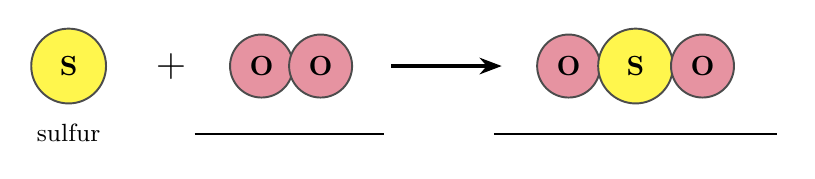
\begin{tikzpicture}[x=1cm, y=1cm]
    \tikzset{S/.style={circle, draw=black!70, fill=yellow!70, line width=0.7pt,
                       minimum size=0.95cm, inner sep=0pt, font=\bfseries},
             O/.style={circle, draw=black!70, fill=cbred!45, line width=0.7pt,
                       minimum size=0.8cm, inner sep=0pt, font=\bfseries}}
    \node[S] at (0,0) {S};
    \node[font=\Large\bfseries] at (1.3,0) {$+$};
    \node[O] at (2.45,0) {O}; \node[O] at (3.2,0) {O};
    \draw[-{Stealth[length=8pt]}, line width=1.2pt] (4.1,0) -- (5.5,0);
    \node[O] at (6.35,0) {O}; \node[S] at (7.2,0) {S}; \node[O] at (8.05,0) {O};
    \node[font=\small] at (0,-0.85) {sulfur};
    \node[font=\small] at (2.8,-0.85) {\blank[2.4cm]};
    \node[font=\small] at (7.2,-0.85) {\blank[3.6cm]};
  \end{tikzpicture}
  \end{center}
  \par\vspace{2pt}
  (a) Write the name of the other reactant, and of the product, under the picture.
  \\[4pt]
  (b) Write the formula of the product. \hfill \blank[2.4cm]
\end{minipage}

\vspace{12pt}
\noindent
\begin{minipage}{\textwidth}
  \textbf{2.} Mr Bowen has two bottles of alkali, \textbf{X} and \textbf{Y}. He puts
  $20\ \ccm$ from one bottle in a flask with a few drops of universal indicator, and
  adds acid until it is neutralised. He does this three times for each bottle.
  \par\vspace{6pt}
  \begin{center}
  \renewcommand{\arraystretch}{1.3}%
  \begin{tabular}{|c|c|c|c|c|}
    \hline
    & \multicolumn{3}{c|}{\textbf{Acid needed in $\mathrm{cm^3}$}} & \\ \cline{2-4}
    \textbf{Bottle} & \textbf{1st try} & \textbf{2nd try} & \textbf{3rd try} &
      \textbf{Mean} \\ \hline
    X & 15 & 16 & 17 & 16 \\ \hline
    Y & 23 & 26 & 23 & \\ \hline
  \end{tabular}
  \end{center}
  \par\vspace{2pt}
  % Full lines rather than short blanks: this page had room to spare, and these
  % are sentence answers.
  (a) How does he know when the alkali has been neutralised?
  \wlines{1}
  (b) Why does he do it three times, not once?
  \wlines{1}
  (c) Work out the mean for bottle \textbf{Y} and write it in the table.
  \par\vspace{10pt}
  (d) Which bottle holds the \textbf{stronger} alkali? Explain how you know.
  \wlines{3}
\end{minipage}

% ===========================================================================
% SECTION D -- BOTH UNITS
% ===========================================================================
\hwsection[cbgreen]{Section D \textperiodcentered\ Both Units}


% -- D1 ---------------------------------------------------------------------
% The deadpan one. Six mistakes, one from almost every lesson, and each has to
% be corrected in a sentence.
\evq{D1}{Mr Bowen's lab notebook}{\challenge}

% One minipage from the instruction to the last line, so the notebook and the
% lines to correct it on cannot be split across a page.
\noindent
\begin{minipage}{\textwidth}
Mr Bowen wrote this. It is full of mistakes. Find \textbf{six}: underline each
one, then write the correct sentence.

\vspace{6pt}
\begin{tcolorbox}[enhanced, colback=black!3, colframe=black!35, boxrule=0.8pt,
                  arc=4pt, left=10pt, right=10pt, top=8pt, bottom=8pt]
  \linespread{1.35}\selectfont
  Monday. I looked at my own cheek cells under the microscope. Each one had a cell
  wall and a big sap vacuole. Their mitochondria make food using sunlight.

  Then I boiled some water for my tea. It boiled at $0\dC$ and turned into water
  vapour, which I could see as a white cloud above the kettle.

  I put salt in my tea. Salt is a mixture of sodium and chlorine. I dipped red
  litmus paper in the salt water and it turned blue, so salt water is an acid.
  The tea was terrible.
\end{tcolorbox}

\vspace{2pt}
\begin{enumerate}[label=\arabic*., itemsep=24pt, topsep=14pt]
  \item {\color{rulegray}\hrulefill}
  \item {\color{rulegray}\hrulefill}
  \item {\color{rulegray}\hrulefill}
  \item {\color{rulegray}\hrulefill}
  \item {\color{rulegray}\hrulefill}
  \item {\color{rulegray}\hrulefill}
\end{enumerate}
\end{minipage}

% ===========================================================================
% ANSWER KEY (teacher copy only)
% ===========================================================================
\ifkey
\newpage
\hwsection[cbred]{Answer Key --- Teacher Copy}

\linespread{1.0}\selectfont
\setlist[enumerate]{itemsep=2pt, topsep=3pt, leftmargin=*}
\setlist[itemize]{itemsep=2pt, topsep=3pt, leftmargin=*}

\noindent{\small A few question \emph{types} here are also on the Quarter 1 Assessment,
at your request; no item is. The list of which is kept with the assessment, not in
this public file. A1, C3, C5(b), C6 and C7 are rewritten from the Cambridge
end-of-year paper.}

\qhead[cbred]{A1}{Every part has a job}
\noindent (a) membrane --- in and out \sep cytoplasm --- chemical reactions \sep
nucleus --- controls everything \sep mitochondrion --- releases energy \sep wall ---
shape \sep chloroplast --- food using sunlight \sep sap vacuole --- cell sap, firm \\
(b) cell wall, chloroplast, sap vacuole

\smallskip
\noindent{\small The membrane and the nucleus swapped is the English trap the word help
names: both jobs start with ``controls''. Mitochondrion to ``makes food'' means
energy and food have become one idea --- the chloroplast \emph{makes} food, the
mitochondrion \emph{releases energy} from it.}

\qhead[cbred]{A2}{The root hair cell}
\noindent (a) 1 cell wall \quad 2 cell membrane \quad 3 cytoplasm \quad 4 nucleus
\quad 5 sap vacuole \quad 6 root hair \\
(b) cell wall 1, cell membrane 2, cytoplasm 3, sap vacuole 4 \\
(c) It gives the cell a big surface, so water can move in easily / it absorbs more
water from the soil.

\smallskip
\noindent{\small (a) 1 and 2 swapped: the wall is the thick green band outside, the
membrane the dark line just inside it. (b) is the 1.3 book question (p.~20 Q4) that no
packet had asked. (c) ``to absorb water'' is the function, not how the shape helps ---
push for ``big surface''.}

\qhead[cbred]{A3}{Which level is it?}
\noindent Cell: neurone, red blood cell \sep Tissue: ciliated epithelium, palisade layer
\sep Organ: brain, root \sep Organ system: digestive, breathing \sep Organism: mango
tree, cat

\smallskip
\noindent{\small The palisade layer (tissue, not cell) and the root (organ --- 1.4 named
roots and flowers as organs) are the two traps.}

\qhead[cbred]{A4}{Mr Bowen's table}
\noindent red blood cell: \emph{very long axon} $\rightarrow$ full of haemoglobin / no
nucleus \sep neurone: \emph{large sap vacuole} $\rightarrow$ a very long axon \sep
ciliated cell: \emph{absorbs water from the soil} $\rightarrow$ sweeps mucus out of the
airways \sep palisade cell: \emph{has no nucleus} $\rightarrow$ packed with chloroplasts


\smallskip
\noindent{\small Row 4 is the hard one: ``no nucleus'' is a real adaptation, just of a
different cell. A student who crosses out the function in row 1 or 2 has not read the
column headings.}

\qhead[cbred]{A5}{Unit 1 puzzles}
\noindent 1. (a) $1 \div 0.02 = \mathbf{50}$ \quad (b) $\mathbf{500}$ \quad
(c) $0.07 \div 0.02 = 3.5$, so \textbf{about 3 or 4} \\
2. A cell wall is stiff and holds the cell in one shape, so the white blood cell could
not change shape to squeeze between cells or wrap around germs.

\smallskip
\noindent{\small 1 is Unit 3 maths: $0.02 \times 50 = 1$. An answer of 0.5 or 5 means
the digits moved the wrong way. 2 is the 1.3 exit question, turned round: a student
who writes ``it has no cell wall'' has described the cell, not answered why.}

\qhead[cbred]{B1}{Draw the particles}
\noindent Solid: touching, in regular rows. Liquid: touching, no pattern. Gas: far
apart, no pattern. Circles the same size in all three.

\qhead[cbred]{B2}{Solid, liquid or gas?}
\noindent own shape: S \sep fills any container: G \sep shape of container, same volume:
L \sep can be poured: \textbf{L and G} \sep cannot be compressed: \textbf{S and L}
\sep vibrate in place: S \sep touch but move past: L

\smallskip
\noindent{\small ``Can be poured'' and ``cannot be compressed'' are the two-tick rows; a
single tick on either is the ``only'' idea not yet understood.}

\qhead[cbred]{B3}{Name the change}
\noindent chocolate: melting, heating \sep breath on a window: condensing, cooling \sep
butter in the fridge: freezing, cooling \sep wet floor: evaporating, heating (from the
air around it) \sep kettle at $100\dC$: boiling, heating

\smallskip
\noindent{\small ``Freezing'' for butter sounds wrong to the class because the fridge is
not below zero --- say so: freezing is liquid to solid, at whatever temperature that
substance does it. Accept ``heating'' or ``neither'' for the floor if explained.}

\qhead[cbred]{B4}{Explain it with particles}
\noindent (a) Heat energy is transferred to the particles. They move faster and faster.
Some escape the attractive forces and leave as a gas (steam / water vapour). \\
(b) There is water vapour in the air. When it touches the cold can, the particles lose
energy and slow down, and the forces pull them together into a liquid: it condenses.

\smallskip
\noindent{\small (b) ``the water comes through the can'' is the misconception: the can is
sealed.}

\qhead[cbred]{B5}{The water cycle}
\noindent 1 evaporation \quad 2 transpiration \quad 3 condensation \quad 4 precipitation
\quad 5 surface run-off \quad 6 groundwater \\
(b) tiny drops of liquid water \quad (c) any two of snow, hail, sleet

\smallskip
\noindent{\small (b) ``water vapour'' is the 2.4 misconception exactly --- a cloud is
drops that have \emph{already} condensed. 1 and 2 swapped: transpiration is water
leaving a plant.}

\qhead[cbred]{B6}{Particle puzzles}
\noindent 1. (a) at 8 minutes (at $100\dC$) \quad (b) $100\dC$ \quad (c) The heat is
changing the liquid into a gas instead of raising the temperature. \\
2. The particles in the water get more energy when it is hot, so they move faster and
more of them escape (evaporate) from the surface.

\smallskip
\noindent{\small 1(b) about $120\dC$ comes from carrying the line on --- the trap the
graph is for. 2: ``the sun dries them'' is not a particle answer.}

\qhead[cbred]{C1}{Symbols, both ways}
\noindent (a) O, K, Mg, Ca, N, Al \quad (b) helium, sulfur, lithium, argon, fluorine,
silicon

\smallskip
\noindent{\small MG, mg or CA: the capital-letter rule. P for potassium is the Latin
trap --- P is phosphorus.}

\qhead[cbred]{C2}{Rows and columns}
\noindent (a) Mg \quad (b) 4 \quad (c) any two of He, Ne, Ar \quad (d) group

\smallskip
\noindent{\small (a) Al or Be: period and group swapped.}

\qhead[cbred]{C3}{Symbols and formulae}
\noindent (a) K and Ca \quad (b) \ch{Cl_2} \quad (c) \ch{CH_4} \quad (d) \ch{K_2CO_3},
potassium carbonate \quad (e) 3 and 6

\smallskip
\noindent{\small (b) is an element even though it has a 2 in it --- the hw07 E4 mistake
again. (e) 5 for \ch{K_2CO_3} means the 2 was not counted.}

\qhead[cbred]{C4}{Naming compounds}
\noindent (a) sodium sulfide, calcium oxide, lithium chloride, magnesium carbonate \\
(b) potassium, nitrogen, oxygen \sep copper, sulfur, oxygen

\smallskip
\noindent{\small (a)2 is written oxygen-first on purpose: ``oxide calcium'' means the
student copied the order instead of putting the metal first.}

\qhead[cbred]{C5}{Element, compound or mixture?}
\noindent (a) 1 E \quad 2 E \quad 3 C \quad 4 M \quad 5 M \quad 6 C \\
(b) element --- one kind of atom \sep compound --- different atoms bonded \sep mixture
--- mixed but not bonded \sep pure --- only one substance \\
(c) with a magnet (iron is magnetic, sand is not) \sep evaporate the water away (heat
it in an evaporating basin)

\smallskip
\noindent{\small Box 2 is the trap: atoms joined in pairs, but all one kind, so an
element (like \ch{O_2}). Box 6 is one substance even though it has two kinds of atom.}

\qhead[cbred]{C6}{Acid or alkali?}
\noindent Acid: tastes sour, pH 2, turns blue litmus red, tamarind, stomach acid,
hydrochloric acid \\
Alkali: pH 12, turns red litmus blue, toothpaste, limewater, sodium hydroxide, baking
soda

\qhead[cbred]{C7}{Two questions from the end of the year}
\noindent 1. (a) reactants: sulfur, oxygen; product: sulfur dioxide \quad (b) \ch{SO_2} \\
2. (a) the universal indicator shows pH 7 (the neutral colour) \quad (b) to check the
results / make them reliable / spot a mistake \quad (c) $(23 + 26 + 23) \div 3 = 72
\div 3 = \mathbf{24}$ \quad (d) Y: it needed more acid to neutralise the same
$20\ \ccm$.

\smallskip
\noindent{\small 2(d) ``X, because 16 is a smaller number'' is the misreading to expect:
the more acid it takes, the stronger the alkali. Do not ask what is made --- the
products are Stage 8.}

\qhead[cbred]{D1}{Mr Bowen's lab notebook}
\begin{enumerate}[label=\arabic*.]
  \item Cheek cells are animal cells: they have no cell wall \dots
  \item \dots and no (large) sap vacuole.
  \item Mitochondria release energy from food; chloroplasts make food (and cheek cells
        have none).
  \item Water boils at $100\dC$, not $0\dC$ (it freezes / melts at 0).
  \item You cannot see water vapour; the white cloud is tiny drops of liquid water.
  \item Salt is a compound (sodium chloride), not a mixture. \quad \emph{Also accept:}
        red litmus turning blue means an alkali, not an acid (salt water is neutral).
\end{enumerate}
\noindent{\small There are seven errors in the text on purpose, so a student who finds a
different six is not penalised. ``The tea was terrible'' is not a mistake.}

\fi

\end{document}
